\documentclass[a4paper,11pt]{article}

% --------------------------------------------
% PACCHETTI
% --------------------------------------------
\usepackage[italian]{babel}
\usepackage{amsmath, amssymb}
\usepackage{graphicx}
\usepackage{geometry}
\usepackage{float}
\usepackage{caption}
\usepackage{xcolor}
\usepackage{titlesec}
\usepackage{parskip}
\usepackage{booktabs}
\usepackage{array}
\usepackage{mdframed}
\usepackage{colortbl}
\usepackage{setspace}
\usepackage{fancyhdr}
\usepackage{lastpage}
\usepackage{tocloft}
\usepackage[T1]{fontenc}
\usepackage{libertinus}
\usepackage{microtype}
\usepackage{tikz}
\usetikzlibrary{arrows.meta, calc, shapes.geometric}

% Override Italian babel: use "Figure" instead of "Figura"
\addto\captionsitalian{\renewcommand{\figurename}{Figure}}

% --------------------------------------------
% MARGINI
% --------------------------------------------
\geometry{a4paper, top=2.8cm, bottom=2.8cm, left=2.8cm, right=2.8cm, headsep=0.7cm}
\setstretch{1.15}

% --------------------------------------------
% COLORI
% --------------------------------------------
\definecolor{epflred}{RGB}{227,6,19}
\definecolor{darkgray}{RGB}{26,26,26}
\definecolor{lightgray}{RGB}{245,245,245}
\definecolor{epflgray}{RGB}{140,140,140}
\definecolor{rowcolor}{RGB}{238,244,250}
\definecolor{warnyellow}{RGB}{255,248,220}
\definecolor{warnborder}{RGB}{210,140,0}
\definecolor{exblue}{RGB}{232,241,252}
\definecolor{exborder}{RGB}{60,120,200}
\definecolor{dipoleblue}{RGB}{30,80,210}
\definecolor{nucleusred}{RGB}{190,30,30}
\definecolor{electronblue}{RGB}{30,100,200}

% --------------------------------------------
% HEADER / FOOTER
% --------------------------------------------
\pagestyle{fancy}
\fancyhf{}
\fancyhead[L]{\small\textcolor{darkgray}{\textsc{Chimica Generale}}\;\textcolor{epflred}{|}\;\textcolor{epflgray}{\textsc{epfl -- cms}}}
\fancyhead[R]{\small\textcolor{epflgray}{\leftmark}}
\fancyfoot[C]{\textcolor{epflgray}{\rule{1.5cm}{0.3pt}}\;\textcolor{epflred}{\textbf{\thepage}}\;\textcolor{epflgray}{\rule{1.5cm}{0.3pt}}}
\renewcommand{\headrulewidth}{0pt}
\renewcommand{\footrulewidth}{0pt}

% --------------------------------------------
% STILE SEZIONI
% --------------------------------------------
\titleformat{\section}
  {\Large\bfseries\color{darkgray}}
  {\colorbox{epflred}{\textcolor{white}{\;\thesection\;}}}{0.7em}{}
  [\vspace{3pt}{\color{epflred}\hrule height 1pt}\vspace{2pt}]

\titleformat{\subsection}
  {\large\bfseries\color{darkgray}}
  {\textcolor{epflred}{\thesubsection}}{0.6em}{}

\titlespacing{\section}{0pt}{22pt}{10pt}
\titlespacing{\subsection}{0pt}{16pt}{6pt}

% --------------------------------------------
% BOX
% --------------------------------------------
\newmdenv[backgroundcolor=lightgray, linecolor=epflred, linewidth=2pt,
  leftline=true, rightline=false, topline=false, bottomline=false,
  innerleftmargin=10pt, innerrightmargin=10pt, innertopmargin=7pt, innerbottommargin=7pt,
  skipabove=8pt, skipbelow=8pt]{definizione}

\newmdenv[backgroundcolor=warnyellow, linecolor=warnborder, linewidth=2pt,
  leftline=true, rightline=false, topline=false, bottomline=false,
  innerleftmargin=10pt, innerrightmargin=10pt, innertopmargin=7pt, innerbottommargin=7pt,
  skipabove=8pt, skipbelow=8pt]{attenzione}

\newmdenv[backgroundcolor=exblue, linecolor=exborder, linewidth=2pt,
  leftline=true, rightline=false, topline=false, bottomline=false,
  innerleftmargin=10pt, innerrightmargin=10pt, innertopmargin=7pt, innerbottommargin=7pt,
  skipabove=8pt, skipbelow=8pt]{esempio}

\newcommand{\altrow}{\rowcolors{2}{rowcolor}{white}}
\newcommand{\resetrow}{\rowcolors{0}{}{}}

% --------------------------------------------
% INDICE
% --------------------------------------------
\renewcommand{\cftsecfont}{\bfseries\color{darkgray}}
\renewcommand{\cftsecpagefont}{\bfseries\color{epflred}}
\renewcommand{\cftsubsecfont}{\color{darkgray}}
\renewcommand{\cftsubsecpagefont}{\color{epflgray}}
\renewcommand{\cftsecleader}{\cftdotfill{\cftdotsep}}
\setlength{\cftbeforesecskip}{4pt}

% ============================================================
\begin{document}
% ============================================================

% COPERTINA
\begin{titlepage}
\centering
\vspace*{3.5cm}

\includegraphics[width=0.65\textwidth]{UNI/Chimica/Logo EPFL 3.jpg}
\vspace{3.5cm}

{\Huge\bfseries\color{darkgray} General Chemestry I}

\vspace{0.55cm}
{\color{epflred}\rule{9cm}{1.8pt}}
\vspace{1.0cm}

{\Large\textsc{\color{darkgray} Course notes}}

\vspace{0.8cm}
{Atomic structure\enspace$\cdot$\enspace molecules\enspace$\cdot$\enspace Bonds}

\vfill
{\color{epflred}\rule{8cm}{0.4pt}}

{\small\color{darkgray}
  \textsc{epfl -- cms}\enspace$\cdot$\enspace  2025--2026\enspace$\cdot$\enspace{\LaTeX}
}
\vspace{2.5cm}
\end{titlepage}

% INDICE
\thispagestyle{empty}
\vspace*{0.5cm}
{\color{epflred}\rule{\textwidth}{1pt}}\par
\vspace{6pt}
\tableofcontents
\clearpage

% ============================================================
\section{Atomic Structure}
% ============================================================

An atom is composed of a \textbf{nucleus} (protons + neutrons) surrounded by an \textbf{electron cloud}. The \textbf{atomic number} $Z$ (= no.\,protons = no.\,electrons for a neutral atom) uniquely identifies the element; the \textbf{mass number} $A$ = protons + neutrons. The notation is ${}^{A}_{Z}X$.

\vspace{4pt}
\altrow
\begin{center}
\begin{tabular}{lccc}
\toprule
\rowcolor{epflred!85}
\textcolor{white}{\textbf{Particle}} & \textcolor{white}{\textbf{Charge}} &
\textcolor{white}{\textbf{Mass (kg)}} & \textcolor{white}{\textbf{Location}} \\
\midrule
Proton    & $+e$ & $1{,}673\times10^{-27}$ & Nucleus \\
Neutron   & $0$  & $1{,}675\times10^{-27}$ & Nucleus \\
Electron  & $-e$ & $9{,}109\times10^{-31}$ & Electron cloud \\
\bottomrule
\end{tabular}
\end{center}
\resetrow

% TikZ: Atom structure
\begin{figure}[H]
\centering
\begin{tikzpicture}[>=Stealth, scale=1.1]
  \shade[ball color=nucleusred!80] (0,0) circle (0.55cm);
  \node[white, font=\footnotesize\bfseries] at (0, 0.14) {p$^+$};
  \node[white, font=\footnotesize\bfseries] at (0,-0.18) {n};
  \node[nucleusred, font=\small\bfseries] at (0,-0.90) {Nucleus};
  % Shell 1
  \draw[epflgray, line width=0.8pt] (0,0) ellipse (1.6cm and 0.5cm);
  \fill[electronblue] ( 1.6, 0) circle (0.13);
  \fill[electronblue] (-1.6, 0) circle (0.13);
  \node[epflgray, font=\scriptsize] at (0, 0.65) {$n=1$};
  % Shell 2
  \draw[epflgray, line width=0.8pt] (0,0) ellipse (2.8cm and 0.9cm);
  \foreach \a in {0,45,90,135,180,225,270,315}
    \fill[electronblue!70] ({2.8*cos(\a)},{0.9*sin(\a)}) circle (0.11);
  \node[epflgray, font=\scriptsize] at (0, 1.05) {$n=2$};
  % Shell 3
  \draw[epflgray, line width=0.6pt, dashed] (0,0) ellipse (4.0cm and 1.35cm);
  \foreach \a in {0,72,144,216,288}
    \fill[electronblue!45] ({4.0*cos(\a)},{1.35*sin(\a)}) circle (0.10);
  \node[epflgray, font=\scriptsize] at (0, 1.52) {$n=3$};
  \node[darkgray, font=\footnotesize] at (4.85, 0) {Electron cloud};
  \draw[->, epflgray, thin] (4.55, 0) -- (3.8, 0.3);
\end{tikzpicture}
\caption{Structure of the atom: nucleus (protons $p^+$ and neutrons $n$) surrounded by electron shells $n=1,2,3,\ldots$}
\end{figure}

\subsection{Isotopes and Atomic Mass}

\begin{definizione}
\textit{Isotopes} are atoms of the same element (same $Z$) with different numbers of neutrons ($n = A - Z$). The \textit{relative atomic mass} is the weighted average of isotope masses over their natural abundances:
\[
M = \sum_i f_i \cdot m_i
\]
where $f_i$ is the fractional abundance and $m_i$ the mass of isotope $i$.
\end{definizione}

\begin{esempio}
$M(\text{Cl}) = 0{,}7577\times34{,}969 + 0{,}2423\times36{,}966 \approx 35{,}45\;\text{u}$
\end{esempio}

\subsection{Mole and Avogadro's Number}

\begin{definizione}
The \textit{mole} (mol) contains exactly $N_A = 6{,}022\times10^{23}$ entities (atoms, molecules, ions\ldots). The \textit{molar mass} $M$ [g/mol] is numerically equal to the atomic mass in u.
\[
n = \frac{m}{M} \qquad N = n\cdot N_A
\]
The mole is the fundamental SI unit of amount of substance.
\end{definizione}

\subsection{Fundamental Laws of Chemistry}

\begin{definizione}
\textbf{Law of Conservation of Mass (Lavoisier)}: in a chemical reaction, the total mass of the reactants is exactly equal to the total mass of the products. Matter is neither created nor destroyed.
\end{definizione}

% TikZ: Lavoisier
\begin{figure}[H]
\centering
\begin{tikzpicture}[>=Stealth, scale=1.0,
  box/.style={draw=epflgray, rounded corners=4pt, fill=lightgray,
              minimum width=2.2cm, minimum height=1.0cm, font=\small, align=center}]
  \node[box, fill=orange!15, draw=orange!60] (Fe) at (-4.5,0) {\textbf{Fe}\\ \small 1.00\,g};
  \node[box, fill=yellow!20, draw=yellow!70!black] (S) at (-2.5,0) {\textbf{S}\\ \small 0.57\,g};
  \node[font=\Large\bfseries, darkgray] at (-1.4,0) {$+$};
  \draw[->, epflred, line width=2pt] (-0.7,0) -- (0.7,0)
    node[above, midway, font=\footnotesize\bfseries, epflred] {reaction};
  \node[box, fill=epflred!12, draw=epflred!60, minimum width=2.6cm] (FeS) at (2.2,0)
    {\textbf{FeS}\\ \small 1.57\,g};
  \draw[darkgray, dashed] (-4.5,-0.75) -- (-4.5,-1.30);
  \draw[darkgray, dashed] (-2.5,-0.75) -- (-2.5,-1.30);
  \draw[<->, darkgray, line width=1pt] (-4.5,-1.25) -- (-2.5,-1.25)
    node[below, midway, font=\scriptsize] {1.00 + 0.57 = 1.57\,g};
  \draw[darkgray, dashed] (2.2,-0.75) -- (2.2,-1.30);
  \node[darkgray, font=\scriptsize] at (2.2,-1.55) {1.57\,g};
  \node[epflred, font=\small\bfseries] at (-1.15,-2.0)
    {$m_{\text{reactants}} = m_{\text{products}}$};
\end{tikzpicture}
\caption{Example of Lavoisier's law: 1\,g of iron + 0{,}57\,g of sulfur $\to$ 1{,}57\,g of iron sulfide.}
\end{figure}

\begin{definizione}
\textbf{Law of Definite Proportions (Proust)}: a chemical compound is always formed by the same elements combined in constant and definite mass ratios.
\end{definizione}

% TikZ: Proust
\begin{figure}[H]
\centering
\begin{tikzpicture}[>=Stealth, scale=1.0,
  box/.style={draw=epflgray, rounded corners=4pt,
              minimum width=2.0cm, minimum height=0.95cm, font=\small, align=center}]
  \node[font=\small\bfseries, epflgray] at (-3.5, 1.6) {Experiment 1};
  \node[box, fill=orange!15, draw=orange!60] at (-4.6,0.6) {\textbf{Fe}\\ \small 10.0\,g};
  \node[font=\normalsize, darkgray] at (-3.35,0.6) {$+$};
  \node[box, fill=yellow!20, draw=yellow!70!black] at (-2.1,0.6) {\textbf{S}\\ \small 5.7\,g};
  \draw[->, epflred, line width=1.8pt] (-0.95,0.6) -- (0.05,0.6);
  \node[box, fill=epflred!12, draw=epflred!60, minimum width=2.4cm] at (1.55,0.6)
    {\textbf{FeS}\\ \small 15.7\,g};
  \node[font=\small\bfseries, epflgray] at (-3.5,-0.8) {Experiment 2};
  \node[box, fill=orange!15, draw=orange!60] at (-4.6,-1.75) {\textbf{Fe}\\ \small 10.0\,g};
  \node[font=\normalsize, darkgray] at (-3.35,-1.75) {$+$};
  \node[box, fill=yellow!20, draw=yellow!70!black, minimum width=2.4cm] at (-1.95,-1.75)
    {\textbf{S}\\ \small 5.7 + 2.3\,g};
  \draw[->, epflred, line width=1.8pt] (-0.75,-1.75) -- (0.05,-1.75);
  \node[box, fill=epflred!12, draw=epflred!60, minimum width=2.4cm] at (1.55,-1.75)
    {\textbf{FeS}\\ \small 15.7\,g};
  \node[box, fill=yellow!35, draw=yellow!80!black] at (4.0,-1.75)
    {\textbf{S}\\ \small 2.3\,g\\ \scriptsize (excess)};
  \draw[epflgray, ->] (2.78,-1.75) -- (3.35,-1.75);
  \draw[darkgray, dashed] (-4.6,-2.55) -- (-4.6,-3.1);
  \draw[darkgray, dashed] (-1.95,-2.55) -- (-1.95,-3.1);
  \node[darkgray, font=\scriptsize] at (-3.3,-3.35)
    {Fixed ratio: $m(\text{Fe})\,{:}\,m(\text{S}) = 10{:}5.7 \approx 1.75$};
\end{tikzpicture}
\caption{Proust's law: 10\,g of iron react with 5{,}7\,g of sulfur; the excess sulfur (2{,}3\,g) does not react.}
\end{figure}

\clearpage

% ============================================================
\section{Electronic Configuration}
% ============================================================

\begin{attenzione}
\textbf{Heisenberg's Uncertainty Principle:} it is impossible to simultaneously know with arbitrary precision both the \textit{position} and the \textit{momentum} of an electron:
\[
\Delta x \cdot \Delta p \;\geq\; \frac{\hbar}{2}
\]
where $\hbar = h/2\pi$ is the reduced Planck constant. There are no well-defined orbits: instead, \textit{orbitals} are used --- regions of space in which the probability of finding the electron is $\geq 90\%$.
\end{attenzione}

\subsection{Quantum Numbers and Orbitals}

\begin{definizione}
An \textit{atomic orbital} is a wave function $\psi_{n,l,m_l}$. Each electron is uniquely described by four quantum numbers:
\begin{itemize}
  \item $n = 1,2,3,\ldots$ \textbf{(principal)}: determines the energy level and average distance from the nucleus.
  \item $l = 0,\ldots,n-1$ \textbf{(azimuthal)}: defines the shape of the orbital ($s,p,d,f$).
  \item $m_l = -l,\ldots,+l$ \textbf{(magnetic)}: specifies the spatial orientation.
  \item $m_s = \pm\tfrac{1}{2}$ \textbf{(spin)}: indicates the intrinsic rotation of the electron.
\end{itemize}
\end{definizione}

\altrow
\begin{center}
\begin{tabular}{ccccc}
\toprule
\rowcolor{epflred!85}
\textcolor{white}{\textbf{Type}} & \textcolor{white}{$l$} &
\textcolor{white}{\textbf{No.\ orbitals}} & \textcolor{white}{\textbf{Max $e^-$}} &
\textcolor{white}{\textbf{Shape}} \\
\midrule
$s$ & 0 & 1 &  2 & Spherical \\
$p$ & 1 & 3 &  6 & Bilobal (3 orientations: $x,y,z$) \\
$d$ & 2 & 5 & 10 & Four-lobed \\
$f$ & 3 & 7 & 14 & Complex \\
\bottomrule
\end{tabular}
\end{center}
\resetrow

The maximum number of electrons per shell $n$ is $2n^2$.

\subsection{Filling Rules}

\begin{definizione}
\textbf{Aufbau Principle}: electrons occupy orbitals in order of increasing energy (Klechkowski rule):
\[
1s < 2s < 2p < 3s < 3p < 4s < 3d < 4p < 5s < 4d < \cdots
\]
\end{definizione}

\begin{definizione}
\textbf{Pauli Exclusion Principle}: no orbital can hold more than two electrons; if two are present, they must have opposite spins.
\end{definizione}

\begin{definizione}
\textbf{Hund's Rule}: among degenerate orbitals, electrons occupy distinct orbitals first with parallel spin, minimizing electrostatic repulsion.
\end{definizione}

\subsection{Notation and Ionic Configuration}

The configuration is written by listing subshells with a superscript for the number of electrons; the preceding noble gas is abbreviated in square brackets. For sulfur ($Z=16$):
\[
1s^2\;2s^2\;2p^6\;3s^2\;3p^4 \;\equiv\; [\text{Ne}]\;3s^2\;3p^4
\]

% TikZ: Electronic configuration diagrams
\begin{figure}[H]
\centering
\begin{tikzpicture}[>=Stealth, scale=1.0,
  orb/.style={draw=darkgray, minimum width=0.52cm, minimum height=0.52cm, inner sep=0pt}]

%% N (Z=7)
\node[darkgray, font=\small\bfseries] at (0, 2.5) {N \;($Z=7$)};
\node[epflgray, font=\scriptsize]     at (0, 2.1) {$1s^2\;2s^2\;2p^3$};
\node[orb] at (-1.7,1.5) {};
  \node[epflred,    font=\bfseries] at (-1.7,1.60) {$\uparrow$};
  \node[electronblue, font=\bfseries] at (-1.7,1.35) {$\downarrow$};
  \node[epflgray,font=\scriptsize] at (-1.7,1.02) {$1s$};
\node[orb] at (-0.6,1.5) {};
  \node[epflred,    font=\bfseries] at (-0.6,1.60) {$\uparrow$};
  \node[electronblue, font=\bfseries] at (-0.6,1.35) {$\downarrow$};
  \node[epflgray,font=\scriptsize] at (-0.6,1.02) {$2s$};
\node[orb] at (0.55,1.5) {}; \node[epflred, font=\bfseries] at (0.55,1.52) {$\uparrow$};
\node[orb] at (1.15,1.5) {}; \node[epflred, font=\bfseries] at (1.15,1.52) {$\uparrow$};
\node[orb] at (1.75,1.5) {}; \node[epflred, font=\bfseries] at (1.75,1.52) {$\uparrow$};
\node[epflgray,font=\scriptsize] at (1.15,1.02) {$2p$};

%% Ar (Z=18)
\node[darkgray, font=\small\bfseries] at (5.5, 2.5) {Ar \;($Z=18$)};
\node[epflgray, font=\scriptsize]     at (5.5, 2.1) {$[\text{Ne}]\;3s^2\;3p^6$};
\node[draw=epflred, rounded corners=3pt, fill=epflred!8,
      font=\scriptsize, inner sep=3pt] at (4.1,1.5) {[Ne]};
\node[orb] at (5.0,1.5) {};
  \node[epflred,    font=\bfseries] at (5.0,1.60) {$\uparrow$};
  \node[electronblue, font=\bfseries] at (5.0,1.35) {$\downarrow$};
  \node[epflgray,font=\scriptsize] at (5.0,1.02) {$3s$};
\node[orb] at (5.90,1.5) {}; \node[epflred,font=\bfseries] at (5.90,1.60) {$\uparrow$}; \node[electronblue,font=\bfseries] at (5.90,1.35) {$\downarrow$};
\node[orb] at (6.50,1.5) {}; \node[epflred,font=\bfseries] at (6.50,1.60) {$\uparrow$}; \node[electronblue,font=\bfseries] at (6.50,1.35) {$\downarrow$};
\node[orb] at (7.10,1.5) {}; \node[epflred,font=\bfseries] at (7.10,1.60) {$\uparrow$}; \node[electronblue,font=\bfseries] at (7.10,1.35) {$\downarrow$};
\node[epflgray,font=\scriptsize] at (6.50,1.02) {$3p$};

%% Sr2+ (Z=38)
\node[darkgray, font=\small\bfseries] at (10.5, 2.5) {Sr$^{2+}$ \;($Z=38$)};
\node[epflgray, font=\scriptsize]     at (10.5, 2.1) {$[\text{Kr}]$ (noble gas config.)};
\node[draw=epflred, rounded corners=3pt, fill=epflred!8,
      font=\scriptsize\bfseries, inner sep=5pt] at (10.5,1.5) {[Kr] --- all subshells full};
\node[epflgray, font=\scriptsize] at (10.5,0.85) {$5s^0$ (both $5s$ electrons removed)};

\draw[epflgray, thin] (3.1,0.5) -- (3.1,2.8);
\draw[epflgray, thin] (8.3,0.5) -- (8.3,2.8);
\end{tikzpicture}
\caption{Filling diagrams for N ($1s^2\,2s^2\,2p^3$, Hund's rule), Ar (complete noble-gas configuration) and Sr$^{2+}$ (isoelectronic with Kr after loss of both $5s$ electrons).}
\end{figure}

\begin{definizione}
\textbf{Cation}: the atom \textit{loses} electrons $\Rightarrow$ positive charge. \textbf{Anion}: the atom \textit{gains} electrons $\Rightarrow$ negative charge. Electrons are always removed from or added to the highest-energy subshell.
\end{definizione}

\begin{esempio}
Fe $(Z{=}26):\;[\text{Ar}]\;3d^6\;4s^2 \;\to\; \text{Fe}^{2+}:\;[\text{Ar}]\;3d^6 \;\to\; \text{Fe}^{3+}:\;[\text{Ar}]\;3d^5$.\\
In transition metals, $4s$ electrons are removed \textit{before} $3d$ electrons.
\end{esempio}

\clearpage

% ============================================================
\section{Periodic Table and Periodic Properties}
% ============================================================

Elements are arranged in order of increasing $Z$. \textbf{Columns} (18 groups) collect elements with the same valence configuration; \textbf{rows} (7 periods) group elements with the same number of occupied shells.

\subsection{Effective Nuclear Charge}

\begin{definizione}
The \textit{effective nuclear charge} $Z_{\text{eff}} = Z - \sigma$ is the charge perceived by the valence electron after \textbf{shielding} $\sigma$ by inner electrons. $Z_{\text{eff}}$ \textbf{increases} across a period and remains \textbf{nearly constant} down a group.
\end{definizione}

\subsection{Periodic Trends}

\altrow
\begin{center}
\begin{tabular}{p{4cm}p{4.5cm}p{4.5cm}}
\toprule
\rowcolor{epflred!85}
\textcolor{white}{\textbf{Property}} &
\textcolor{white}{\textbf{Across period ($\rightarrow$)}} &
\textcolor{white}{\textbf{Down group ($\downarrow$)}} \\
\midrule
Atomic radius & Decreases & Increases \\
Ionization energy & Increases & Decreases \\
Electron affinity & Increases & Decreases \\
Electronegativity (Pauling scale) & Increases (max F $= 4{,}0$) & Decreases (min Cs $= 0{,}79$) \\
Metallic character & Decreases & Increases \\
\bottomrule
\end{tabular}
\end{center}
\resetrow

\begin{figure}[H]
  \centering
  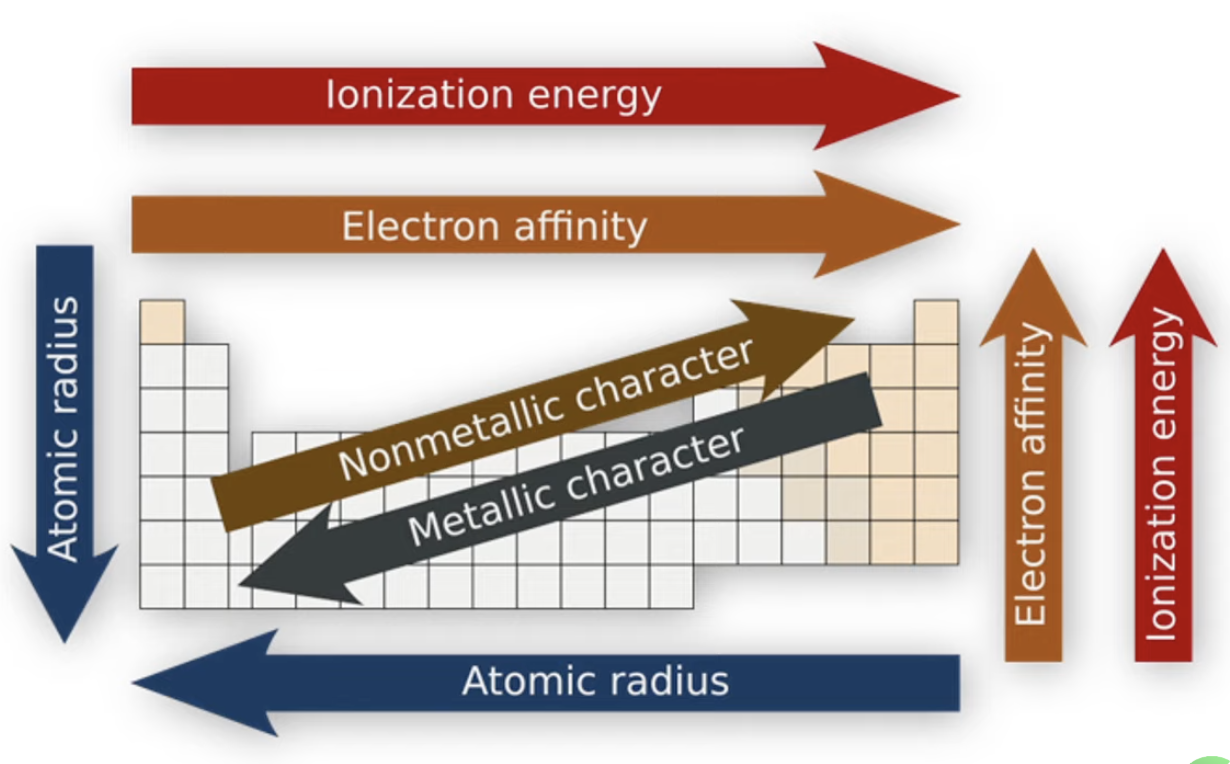
\includegraphics[width=0.55\textwidth]{IMG.2 .png}
  \caption{Summary of the main periodic trends.}
\end{figure}

\clearpage

% ============================================================
\section{Molecular Geometry and Polarity}
% ============================================================

\subsection{VSEPR Theory}

\begin{definizione}
The \textbf{VSEPR} theory (\textit{Valence-Shell Electron-Pair Repulsion}) states that electron pairs around a central atom --- both bonding and lone pairs --- arrange themselves in space to \textbf{minimise mutual repulsion}, maximising the angular distance between them.
\end{definizione}

The notation $\mathrm{A}\,X_n\,E_m$ describes the central atom A with $n$ bonded atoms X and $m$ lone pairs E. Lone pairs occupy more angular space than bonding pairs and \textbf{compress} bond angles.

\vspace{4pt}
\altrow
\begin{center}
\begin{tabular}{lllll}
\toprule
\rowcolor{epflred!85}
\textcolor{white}{\textbf{AXE}} &
\textcolor{white}{\textbf{El.\ gr.}} &
\textcolor{white}{\textbf{Molecular geometry}} &
\textcolor{white}{\textbf{Angle}} &
\textcolor{white}{\textbf{Example}} \\
\midrule
$\mathrm{AX_2E_0}$ & 2 & Linear                    & $180°$        & BeH$_2$, CO$_2$ \\
$\mathrm{AX_3E_0}$ & 3 & Trigonal planar            & $120°$        & BH$_3$, BF$_3$ \\
$\mathrm{AX_4E_0}$ & 4 & Tetrahedral                & $109{,}5°$    & CH$_4$ \\
$\mathrm{AX_3E_1}$ & 4 & Trigonal pyramidal         & $107{,}3°$    & NH$_3$ \\
$\mathrm{AX_2E_2}$ & 4 & Bent                       & $105°$        & H$_2$O \\
$\mathrm{AX_5E_0}$ & 5 & Trigonal bipyramidal       & $90°/120°$    & PCl$_5$ \\
$\mathrm{AX_6E_0}$ & 6 & Octahedral                 & $90°$         & SF$_6$ \\
\bottomrule
\end{tabular}
\end{center}
\resetrow

\begin{figure}[H]
\centering
\begin{tikzpicture}[>=Stealth, scale=0.88,
  central/.style={circle, fill=epflred!75, draw=epflred!90!black,
                  minimum size=0.70cm, font=\small\bfseries, text=white},
  ligand/.style={circle, fill=gray!35, draw=gray!55,
                 minimum size=0.55cm, font=\scriptsize\bfseries, text=darkgray},
  lp/.style={ellipse, fill=gray!20, draw=gray!45, dashed,
             minimum width=0.60cm, minimum height=0.30cm}]

\begin{scope}[xshift=0cm]
  \node[central] (A1) at (0,0) {A};
  \node[ligand] at (-1.4,0) {X}; \node[ligand] at (1.4,0) {X};
  \draw[line width=1.8pt] (A1)--(-1.4,0); \draw[line width=1.8pt] (A1)--(1.4,0);
  \node[font=\scriptsize\bfseries, epflred] at (0,-0.55) {$180°$};
  \node[font=\scriptsize, epflgray] at (0,-0.95) {Linear};
  \node[font=\scriptsize, darkgray] at (0,-1.28) {AX$_2$E$_0$};
\end{scope}

\begin{scope}[xshift=4.0cm]
  \node[central] (A2) at (0,0) {A};
  \node[ligand] at (0,1.30) {X}; \node[ligand] at (-1.12,-0.65) {X}; \node[ligand] at (1.12,-0.65) {X};
  \draw[line width=1.8pt] (A2)--(0,1.30); \draw[line width=1.8pt] (A2)--(-1.12,-0.65); \draw[line width=1.8pt] (A2)--(1.12,-0.65);
  \node[font=\scriptsize\bfseries, epflred] at (0,-1.15) {$120°$};
  \node[font=\scriptsize, epflgray] at (0,-1.50) {Trigonal pl.};
  \node[font=\scriptsize, darkgray] at (0,-1.82) {AX$_3$E$_0$};
\end{scope}

\begin{scope}[xshift=8.0cm]
  \node[central] (A3) at (0,0) {A};
  \node[ligand] at (0,1.32) {X}; \node[ligand] at (-1.12,-0.62) {X}; \node[ligand] at (1.12,-0.62) {X}; \node[ligand] at (0.55,0.30) {X};
  \draw[line width=1.8pt] (A3)--(0,1.32); \draw[line width=1.8pt] (A3)--(-1.12,-0.62); \draw[line width=1.8pt] (A3)--(1.12,-0.62); \draw[line width=1.8pt,dashed] (A3)--(0.55,0.30);
  \node[font=\scriptsize\bfseries, epflred] at (0,-1.10) {$109{,}5°$};
  \node[font=\scriptsize, epflgray] at (0,-1.45) {Tetrahedral};
  \node[font=\scriptsize, darkgray] at (0,-1.78) {AX$_4$E$_0$};
\end{scope}

\begin{scope}[xshift=12.0cm]
  \node[lp] at (0,1.15) {}; \fill[darkgray] (-0.10,1.12) circle(0.06); \fill[darkgray] (0.10,1.12) circle(0.06);
  \node[central] (A4) at (0,0.20) {A};
  \node[ligand] at (-1.10,-0.80) {X}; \node[ligand] at (0,-1.15) {X}; \node[ligand] at (1.10,-0.80) {X};
  \draw[line width=1.8pt] (A4)--(-1.10,-0.80); \draw[line width=1.8pt] (A4)--(0,-1.15); \draw[line width=1.8pt] (A4)--(1.10,-0.80);
  \node[font=\scriptsize\bfseries, epflred] at (0,-1.58) {$107{,}3°$};
  \node[font=\scriptsize, epflgray] at (0,-1.92) {Pyramidal};
  \node[font=\scriptsize, darkgray] at (0,-2.25) {AX$_3$E$_1$};
\end{scope}

\begin{scope}[xshift=0cm, yshift=-5.0cm]
  \node[lp, minimum width=0.55cm] at (-0.18,1.05) {}; \node[lp, minimum width=0.55cm] at (0.18,1.05) {};
  \fill[darkgray] (-0.30,1.05) circle (0.06); \fill[darkgray] (-0.10,1.05) circle (0.06);
  \fill[darkgray] (0.10,1.05) circle (0.06); \fill[darkgray] (0.30,1.05) circle (0.06);
  \node[central] (A5) at (0,0) {A};
  \node[ligand] at (-1.15,-0.88) {X}; \node[ligand] at (1.15,-0.88) {X};
  \draw[line width=1.8pt] (A5)--(-1.15,-0.88); \draw[line width=1.8pt] (A5)--(1.15,-0.88);
  \draw[epflred, line width=1.0pt] (-0.72,-0.55) arc[start angle=220, end angle=320, radius=0.90];
  \node[font=\scriptsize\bfseries, epflred] at (0,-1.42) {$105°$};
  \node[font=\scriptsize, epflgray] at (0,-1.78) {Bent};
  \node[font=\scriptsize, darkgray] at (0,-2.10) {AX$_2$E$_2$};
\end{scope}

\begin{scope}[xshift=4.0cm, yshift=-5.0cm]
  \node[central] (A6) at (0,0) {A};
  \node[ligand] at (0,1.35) {X}; \node[ligand] at (0,-1.35) {X}; \node[ligand] at (-1.25,0) {X};
  \node[ligand] at (0.62,1.08) {X}; \node[ligand] at (0.62,-1.08) {X};
  \draw[line width=1.8pt] (A6)--(0,1.35); \draw[line width=1.8pt] (A6)--(0,-1.35); \draw[line width=1.8pt] (A6)--(-1.25,0);
  \draw[line width=1.8pt,dashed] (A6)--(0.62,1.08); \draw[line width=1.8pt,dashed] (A6)--(0.62,-1.08);
  \node[font=\scriptsize\bfseries, epflred] at (0,-1.82) {$90°/120°$};
  \node[font=\scriptsize, epflgray] at (0,-2.15) {Trigonal bipyram.};
  \node[font=\scriptsize, darkgray] at (0,-2.48) {AX$_5$E$_0$};
\end{scope}

\begin{scope}[xshift=8.0cm, yshift=-5.0cm]
  \node[central] (A7) at (0,0) {A};
  \node[ligand] at (0,1.30) {X}; \node[ligand] at (0,-1.30) {X}; \node[ligand] at (-1.30,0) {X}; \node[ligand] at (1.30,0) {X};
  \node[ligand] at (0.55,0.55) {X}; \node[ligand] at (-0.55,-0.55) {X};
  \draw[line width=1.8pt] (A7)--(0,1.30); \draw[line width=1.8pt] (A7)--(0,-1.30);
  \draw[line width=1.8pt] (A7)--(-1.30,0); \draw[line width=1.8pt] (A7)--(1.30,0);
  \draw[line width=1.8pt,dashed] (A7)--(0.55,0.55); \draw[line width=1.8pt,dashed] (A7)--(-0.55,-0.55);
  \node[font=\scriptsize\bfseries, epflred] at (0,-1.78) {$90°$};
  \node[font=\scriptsize, epflgray] at (0,-2.10) {Octahedral};
  \node[font=\scriptsize, darkgray] at (0,-2.42) {AX$_6$E$_0$};
\end{scope}

\end{tikzpicture}
\caption{Main molecular geometries according to VSEPR theory. Lone pairs (E) are shown as dashed ellipses and compress bond angles.}
\end{figure}

\subsection{Polarity of Molecules}

\begin{definizione}
A molecule is \textbf{polar} when it possesses a \textbf{permanent non-zero dipole moment} ($\vec{\mu}_{\text{tot}} \neq 0$): there is a persistent net separation of positive ($\delta^+$) and negative ($\delta^-$) charge. Two conditions must be satisfied \textit{simultaneously}:
\begin{enumerate}
  \item \textbf{Polar bonds}: the bonded atoms have a significant $\Delta EN$, generating partial bond dipoles ($\vec{\mu}_i$).
  \item \textbf{Asymmetric geometry}: the vector sum of the individual $\vec{\mu}_i$ does not cancel, yielding $\vec{\mu}_{\text{tot}} \neq \vec{0}$.
\end{enumerate}
If the geometry is symmetric, even polar bonds can give $\vec{\mu}_{\text{tot}} = 0$ (\textbf{nonpolar} molecule).
\end{definizione}

\vspace{8pt}

\begin{figure}[H]
\centering
\begin{tikzpicture}[scale=1.05, >=Stealth]

\begin{scope}[xshift=0cm]
  \filldraw[fill=epflred!65, draw=epflred!90!black] (-2.0,0) circle (0.42);
  \node[white, font=\small\bfseries] at (-2.0,0) {O};
  \filldraw[fill=gray!55, draw=gray!70] (0,0) circle (0.32);
  \node[white, font=\small\bfseries] at (0,0) {C};
  \filldraw[fill=epflred!65, draw=epflred!90!black] (2.0,0) circle (0.42);
  \node[white, font=\small\bfseries] at (2.0,0) {O};
  \draw[line width=1.6pt] (-1.58,0.10)--(-0.32,0.10); \draw[line width=1.6pt] (-1.58,-0.10)--(-0.32,-0.10);
  \draw[line width=1.6pt] (0.32,0.10)--(1.58,0.10);   \draw[line width=1.6pt] (0.32,-0.10)--(1.58,-0.10);
  \node[epflred, font=\normalsize\bfseries] at (-2.0,0.78) {$\delta^{-}$};
  \node[epflred, font=\normalsize\bfseries] at (0.0,-0.68) {$\delta^{+}$};
  \node[epflred, font=\normalsize\bfseries] at (2.0,0.78) {$\delta^{-}$};
  \draw[->, dipoleblue, line width=1.6pt] (-0.55,1.00)--(-1.65,1.00) node[above,midway,font=\footnotesize\bfseries,dipoleblue]{$\vec{\mu}_1$};
  \draw[->, dipoleblue, line width=1.6pt] (0.55,1.00)--(1.65,1.00) node[above,midway,font=\footnotesize\bfseries,dipoleblue]{$\vec{\mu}_2$};
  \node[font=\small\bfseries, darkgray] at (0,-1.25) {$\vec{\mu}_1 + \vec{\mu}_2 = \vec{0}$};
  \node[font=\small, epflgray] at (0,-1.72) {linear, symmetric};
  \draw[rounded corners=5pt, warnborder, line width=1.0pt, dashed] (-2.85,-2.1) rectangle (2.85,1.62);
  \node[warnborder, font=\small\bfseries] at (0,2.00) {CO$_2$ --- no net dipole};
\end{scope}

\begin{scope}[xshift=7.6cm]
  \filldraw[fill=epflred!80, draw=epflred!90!black] (0,0.30) circle (0.44);
  \node[white, font=\small\bfseries] at (0,0.30) {O};
  \fill[darkgray] (-0.38,0.88) circle (0.055); \fill[darkgray] (-0.22,0.94) circle (0.055);
  \fill[darkgray] (0.38,0.88) circle (0.055);  \fill[darkgray] (0.22,0.94) circle (0.055);
  \filldraw[fill=gray!15, draw=gray!55] (-1.18,-0.88) circle (0.28);
  \node[darkgray, font=\small\bfseries] at (-1.18,-0.88) {H};
  \filldraw[fill=gray!15, draw=gray!55] (1.18,-0.88) circle (0.28);
  \node[darkgray, font=\small\bfseries] at (1.18,-0.88) {H};
  \draw[line width=2pt] (-0.32,-0.04)--(-0.92,-0.64); \draw[line width=2pt] (0.32,-0.04)--(0.92,-0.64);
  \node[epflred, font=\normalsize\bfseries] at (0.0,0.98) {$\delta^{-}$};
  \node[epflred, font=\small\bfseries] at (-1.68,-0.88) {$\delta^{+}$};
  \node[epflred, font=\small\bfseries] at (1.68,-0.88) {$\delta^{+}$};
  \draw[->, dipoleblue!45, line width=1.2pt] (-0.80,-0.52)--(-0.18,0.05);
  \draw[->, dipoleblue!45, line width=1.2pt] (0.80,-0.52)--(0.18,0.05);
  \draw[->, dipoleblue, ultra thick, line width=2.4pt] (0,0.82)--(0,2.05) node[right=2pt,font=\small\bfseries,dipoleblue]{$\vec{\mu}_{\text{tot}}$};
  \node[font=\small\bfseries, darkgray] at (0,-1.65) {$\vec{\mu}_{\text{tot}} \neq \vec{0}$};
  \node[font=\small, epflgray] at (0,-2.10) {bent, asymmetric};
  \draw[rounded corners=5pt, exborder, line width=1.0pt, dashed] (-2.35,-2.45) rectangle (2.35,2.40);
  \node[exborder, font=\small\bfseries] at (0,2.78) {H$_2$O --- permanent dipole};
\end{scope}

\end{tikzpicture}
\caption{Comparison between a nonpolar molecule (CO$_2$, linear) and a polar molecule (H$_2$O, bent). In CO$_2$ the two dipoles cancel by symmetry; in H$_2$O the bent geometry produces a net dipole directed towards oxygen ($\delta^-$).}
\end{figure}

\vspace{4pt}
\altrow
\begin{center}
\begin{tabular}{p{5.5cm}p{7cm}}
\toprule
\rowcolor{epflred!85}
\textcolor{white}{\textbf{Nonpolar ($\vec{\mu}_{\text{tot}}=0$)}} &
\textcolor{white}{\textbf{Polar ($\vec{\mu}_{\text{tot}}\neq 0$)}} \\
\midrule
Polar bonds present, but the vector sum cancels by symmetry. &
Asymmetric geometry: the resultant of the bond dipoles is non-zero. \\[4pt]
\textit{E.g.}\ CO$_2$ (linear): the two $\vec{\mu}$(C=O) oppose each other. &
\textit{E.g.}\ H$_2$O (bent): the two $\vec{\mu}$(O--H) do not cancel. \\
\textit{E.g.}\ CCl$_4$ (symmetric tetrahedral): $\vec{\mu}_{\text{tot}} = 0$. &
\textit{E.g.}\ NH$_3$ (pyramidal), HCl (heteronuclear diatomic), HF. \\
\bottomrule
\end{tabular}
\end{center}
\resetrow

\begin{attenzione}
A nonpolar bond ($\Delta EN \approx 0$) does not contribute to the dipole moment. Molecular polarity requires \emph{both} polar bonds \emph{and} asymmetric geometry: polar bonds alone are insufficient if the geometry is symmetric (as in CCl$_4$). Polarity also determines \textbf{solubility}: \textit{like dissolves like} --- polar solvents dissolve polar or ionic substances; nonpolar solvents dissolve nonpolar substances.
\end{attenzione}

\clearpage

% ============================================================
\section{Lewis Structure}
% ============================================================

A Lewis structure is a graphical representation showing the distribution of \textbf{valence electrons} in a molecule or polyatomic ion. Bonds are indicated by dashes (each dash = 2 shared electrons), lone pairs by pairs of dots.

\begin{definizione}
A \textbf{Lewis structure} is a representation that makes explicit:
\begin{itemize}
  \item all \textbf{covalent bonds} between atoms (single, double or triple);
  \item all \textbf{lone pairs} (not involved in bonding);
  \item the \textbf{formal charge} (FC) of each atom:
  \[
    \text{FC} = (\text{valence electrons}) - (\text{lone electrons}) - \tfrac{1}{2}(\text{bonding electrons})
  \]
\end{itemize}
The most stable structure minimises formal charges (ideally FC\,$= 0$) and, if residual, assigns negative charges to the most electronegative atoms.
\end{definizione}

\noindent Atoms tend to satisfy the \textbf{octet rule} ($ns^2np^6$, 8 valence electrons); H and He follow the \textbf{duet rule} ($1s^2$, 2 electrons).

\vspace{6pt}
\textbf{Step-by-step procedure:}
\begin{enumerate}
  \item \textbf{Count} the total valence electrons.
  \item \textbf{Build the skeleton}: least electronegative atom is central; H and F always peripheral.
  \item \textbf{Complete the octets} of peripheral atoms.
  \item \textbf{Place remaining electrons} on the central atom as lone pairs.
  \item \textbf{Check the central octet}: if incomplete, convert lone pairs into multiple bonds.
  \item \textbf{Calculate formal charges} and select the most stable structure.
\end{enumerate}

\begin{figure}[H]
\centering
\begin{tikzpicture}[>=Stealth, scale=1.0,
  atomO/.style={circle, minimum size=0.7cm, inner sep=0pt, font=\small\bfseries, fill=epflred!80, draw=epflred!90!black, text=white},
  atomC/.style={circle, minimum size=0.7cm, inner sep=0pt, font=\small\bfseries, fill=gray!65, draw=gray!80, text=white},
  atomH/.style={circle, minimum size=0.6cm, inner sep=0pt, font=\small\bfseries, fill=gray!30, draw=gray!60, text=darkgray},
  atomN/.style={circle, minimum size=0.7cm, inner sep=0pt, font=\small\bfseries, fill=blue!55, draw=blue!70, text=white}]

\begin{scope}[xshift=0cm]
  \draw[rounded corners=6pt, gray!40, line width=0.8pt] (-2.0,-2.2) rectangle (2.0,2.2);
  \node[epflred, font=\small\bfseries] at (0,1.92) {H$_2$O};
  \node[atomO] (O) at (0,0) {O};
  \node[atomH] (H1) at (-1.1,-1.0) {H}; \node[atomH] (H2) at (1.1,-1.0) {H};
  \draw[line width=1.8pt] (O)--(H1); \draw[line width=1.8pt] (O)--(H2);
  \fill[darkgray] (-0.28,0.52) circle (0.06); \fill[darkgray] (-0.12,0.58) circle (0.06);
  \fill[darkgray] (0.12,0.58) circle (0.06); \fill[darkgray] (0.28,0.52) circle (0.06);
  \node[epflgray, font=\scriptsize] at (0,-1.78) {AX$_2$E$_2$ --- bent, $105°$};
\end{scope}

\begin{scope}[xshift=5.2cm]
  \draw[rounded corners=6pt, gray!40, line width=0.8pt] (-2.3,-2.2) rectangle (2.3,2.2);
  \node[epflred, font=\small\bfseries] at (0,1.92) {CO$_2$};
  \node[atomC] (C) at (0,0) {C};
  \node[atomO] (OL) at (-1.7,0) {O}; \node[atomO] (OR) at (1.7,0) {O};
  \draw[line width=1.8pt] (-0.35,0.08)--(-1.35,0.08); \draw[line width=1.8pt] (-0.35,-0.08)--(-1.35,-0.08);
  \draw[line width=1.8pt] (0.35,0.08)--(1.35,0.08);   \draw[line width=1.8pt] (0.35,-0.08)--(1.35,-0.08);
  \fill[darkgray] (-1.90,0.28) circle (0.06); \fill[darkgray] (-2.02,0.14) circle (0.06);
  \fill[darkgray] (-1.90,-0.28) circle (0.06); \fill[darkgray] (-2.02,-0.14) circle (0.06);
  \fill[darkgray] (1.90,0.28) circle (0.06); \fill[darkgray] (2.02,0.14) circle (0.06);
  \fill[darkgray] (1.90,-0.28) circle (0.06); \fill[darkgray] (2.02,-0.14) circle (0.06);
  \node[darkgray, font=\small\bfseries] at (0,-1.35) {$\vec{\mu}_{\text{tot}} = \vec{0}$};
  \node[epflgray, font=\scriptsize] at (0,-1.78) {AX$_2$E$_0$ --- linear, $180°$};
\end{scope}

\begin{scope}[xshift=10.6cm]
  \draw[rounded corners=6pt, gray!40, line width=0.8pt] (-2.0,-2.2) rectangle (2.0,2.2);
  \node[epflred, font=\small\bfseries] at (0,1.92) {NH$_3$};
  \node[atomN] (N) at (0,0.1) {N};
  \node[atomH] (Ha) at (-1.0,-1.0) {H}; \node[atomH] (Hb) at (0.0,-1.3) {H}; \node[atomH] (Hc) at (1.0,-1.0) {H};
  \draw[line width=1.8pt] (N)--(Ha); \draw[line width=1.8pt] (N)--(Hb); \draw[line width=1.8pt] (N)--(Hc);
  \fill[darkgray] (-0.12,0.72) circle (0.07); \fill[darkgray] (0.12,0.72) circle (0.07);
  \node[epflgray, font=\scriptsize] at (0,-1.78) {AX$_3$E$_1$ --- pyramidal, $107°$};
\end{scope}

\end{tikzpicture}
\caption{Lewis structures for H$_2$O, CO$_2$ and NH$_3$. Dots indicate lone pairs.}
\end{figure}

\begin{attenzione}
\textbf{Exceptions to the octet rule.}
\begin{itemize}
  \item \textit{Incomplete octet}: BF$_3$ (B has only 6 $e^-$), BeH$_2$ (Be has 4 $e^-$). These atoms are electrophilic.
  \item \textit{Expanded octet}: SF$_6$, PCl$_5$, XeF$_4$. Third-period elements use vacant $3d$ orbitals.
  \item \textit{Radicals}: NO, NO$_2$. Odd number of $e^-$, paramagnetic.
\end{itemize}
\end{attenzione}

\textbf{Resonance structures.} When multiple equivalent Lewis structures describe the same molecule, the real molecule is a \textit{resonance hybrid} with bonds of intermediate length and energy. Example: CO$_3^{2-}$ has three equivalent resonance structures; C--O bond order $= 4/3 \approx 1{,}33$.

\begin{esempio}
\textbf{H$_2$O}: valence $e^- = 2\!\times\!1 + 6 = 8$. Geometry $\mathrm{AX_2E_2}$ $\Rightarrow$ \textbf{bent}, $105°$.\\
\textbf{CO$_2$}: valence $e^- = 4 + 2\!\times\!6 = 16$. Two double bonds. Geometry \textbf{linear}, $180°$.\\
\textbf{AsCl$_3$}: valence $e^- = 5 + 3\!\times\!7 = 26$. Geometry $\mathrm{AX_3E_1}$ $\Rightarrow$ \textbf{trigonal pyramidal}.
\end{esempio}

\clearpage

% ============================================================
\section{Chemical Bonds}
% ============================================================

\begin{definizione}
A \textit{chemical bond} is an electrical interaction that holds atoms together in a molecule or solid. The type of bond depends mainly on the \textbf{electronegativity difference} $\Delta EN$ between the atoms involved:
\begin{itemize}
  \item \textbf{Intramolecular bonds}: hold atoms together \textit{within} a molecule. Typical energies: 150--1000\,kJ\,mol$^{-1}$.
  \item \textbf{Intermolecular bonds}: act \textit{between} distinct molecules. Typical energies: 0{,}1--40\,kJ\,mol$^{-1}$.
\end{itemize}
\end{definizione}

\subsection{Intramolecular Bonds}

\altrow
\begin{center}
\begin{tabular}{lllll}
\toprule
\rowcolor{epflred!85}
\textcolor{white}{\textbf{Type}} & \textcolor{white}{$\Delta EN$} & \textcolor{white}{\textbf{Description}} & \textcolor{white}{\textbf{Energy}} & \textcolor{white}{\textbf{Example}} \\
\midrule
Nonpolar covalent & $\approx 0$             & Symmetric $e^-$ sharing     & 150--500\,kJ/mol  & Cl$_2$, O$_2$ \\
Polar covalent    & $0 < \Delta EN \leq 1{,}7$ & Asymmetric sharing, dipole & 200--600\,kJ/mol  & HCl, H$_2$O \\
Ionic             & $\Delta EN > 1{,}7$     & $e^-$ transfer, ions formed & 400--1000\,kJ/mol & NaCl, MgO \\
Metallic          & $\approx 0$ (metals)    & Delocalised $e^-$ lattice   & 75--900\,kJ/mol   & Fe, Cu, Au \\
\bottomrule
\end{tabular}
\end{center}
\resetrow

\subsubsection*{Covalent Bond}

The \textit{covalent bond} consists of the \textbf{sharing} of one or more electron pairs. Single bond = 1$\sigma$; double = 1$\sigma$ + 1$\pi$; triple = 1$\sigma$ + 2$\pi$.

\begin{figure}[H]
\centering
\begin{tikzpicture}[>=Stealth, scale=1.0]
\begin{scope}[xshift=0cm]
  \draw[rounded corners=5pt, gray!35, line width=0.8pt] (-2.6,-1.7) rectangle (2.6,1.9);
  \node[epflred, font=\small\bfseries] at (0,1.62) {Nonpolar covalent};
  \draw[green!45!black!25, line width=0.8pt, dashed] (-1.9,0) circle (1.2);
  \draw[green!45!black!25, line width=0.8pt, dashed] (1.9,0) circle (1.2);
  \node[circle, fill=green!55!black, draw=green!75!black, minimum size=0.80cm, font=\small\bfseries, text=white] at (-1.9,0) {Cl};
  \node[circle, fill=green!55!black, draw=green!75!black, minimum size=0.80cm, font=\small\bfseries, text=white] at (1.9,0) {Cl};
  \draw[line width=2.2pt] (-1.50,0)--(1.50,0);
  \fill[darkgray] (-0.12,0.13) circle (0.07); \fill[darkgray] (0.12,0.13) circle (0.07);
  \node[epflgray, font=\scriptsize] at (0,-1.42) {Cl--Cl,\;$\Delta EN = 0$};
\end{scope}
\begin{scope}[xshift=6.6cm]
  \draw[rounded corners=5pt, gray!35, line width=0.8pt] (-2.6,-1.7) rectangle (2.6,1.9);
  \node[epflred, font=\small\bfseries] at (0,1.62) {Polar covalent};
  \draw[gray!40, line width=0.8pt, dashed] (-1.4,0) circle (0.90);
  \draw[purple!35, line width=0.8pt, dashed] (1.4,0) circle (1.20);
  \node[circle, fill=gray!50, draw=gray!65, minimum size=0.68cm, font=\small\bfseries, text=white] at (-1.4,0) {H};
  \node[circle, fill=purple!60, draw=purple!80, minimum size=0.84cm, font=\small\bfseries, text=white] at (1.4,0) {F};
  \draw[line width=2.2pt] (-1.05,0)--(1.01,0);
  \fill[darkgray] (1.72,0.27) circle (0.06); \fill[darkgray] (1.86,0.13) circle (0.06);
  \fill[darkgray] (1.72,-0.27) circle (0.06); \fill[darkgray] (1.86,-0.13) circle (0.06);
  \node[dipoleblue, font=\footnotesize\bfseries] at (-1.4,0.78) {$\delta^+$};
  \node[epflred,   font=\footnotesize\bfseries] at (1.4,0.90) {$\delta^-$};
  \draw[->, dipoleblue, line width=1.6pt] (-0.90,0.52)--(0.90,0.52) node[above,midway,font=\scriptsize\bfseries,dipoleblue]{$\vec{\mu}$};
  \node[epflgray, font=\scriptsize] at (0,-1.42) {H--F,\;$\Delta EN = 1{,}78$};
\end{scope}
\end{tikzpicture}
\caption{Nonpolar covalent bond (Cl$_2$) and polar covalent bond (HF).}
\end{figure}

\subsubsection*{Ionic Bond}

Forms when $\Delta EN > 1{,}7$: the metal \textbf{donates} electrons (cation), the non-metal \textbf{accepts} them (anion). The lattice energy is:
\[
U \propto \frac{|z^+|\cdot|z^-|}{r^+ + r^-}
\]

\begin{esempio}
\textbf{NaCl}: $\Delta EN = 3{,}16 - 0{,}93 = 2{,}23 \;\Rightarrow\;$ Na$^+$ [conf.\ Ne] $+$ Cl$^-$ [conf.\ Ar].
\end{esempio}

% TikZ: Ion formation
\begin{figure}[H]
\centering
\begin{tikzpicture}[>=Stealth, scale=1.0]

% --- Column 1: Neutral atoms ---
\node[font=\small\bfseries, epflgray] at (-4.5, 3.0) {Neutral atoms};
\node[circle, fill=nucleusred!75, draw=nucleusred!90, minimum size=0.70cm, font=\small\bfseries, text=white] at (-4.5, 1.8) {A};
\draw[electronblue!50, thin] (-4.5,1.8) ellipse (1.1 and 0.4);
\draw[electronblue!50, thin] (-4.5,1.8) ellipse (0.5 and 0.9);
\foreach \a in {0,120,240} \fill[electronblue!80] ({-4.5+1.1*cos(\a)},{1.8+0.4*sin(\a)}) circle (0.08);
\node[circle, fill=nucleusred!75, draw=nucleusred!90, minimum size=0.70cm, font=\small\bfseries, text=white] at (-4.5,-0.5) {B};
\draw[electronblue!50, thin] (-4.5,-0.5) ellipse (1.2 and 0.45);
\draw[electronblue!50, thin] (-4.5,-0.5) ellipse (0.55 and 1.0);
\foreach \a in {0,72,144,216,288} \fill[electronblue!80] ({-4.5+1.2*cos(\a)},{-0.5+0.45*sin(\a)}) circle (0.08);

% --- Column 2: Transfer ---
\node[font=\small\bfseries, epflgray] at (0, 3.0) {Electron transfer};
\node[font=\scriptsize, epflgray, align=center] at (0,-1.55) {energy input required};
\draw[epflred, line width=1.6pt] (-0.15,-1.15)--(0.10,-0.70)--(-0.05,-0.70)--(0.20,-0.25);
\node[circle, fill=nucleusred!75, draw=nucleusred!90, minimum size=0.70cm, font=\small\bfseries, text=white] at (0, 1.8) {A};
\draw[electronblue!50, thin] (0,1.8) ellipse (1.1 and 0.4);
\draw[electronblue!50, thin] (0,1.8) ellipse (0.5 and 0.9);
\foreach \a in {120,240} \fill[electronblue!80] ({0+1.1*cos(\a)},{1.8+0.4*sin(\a)}) circle (0.08);
\fill[epflred!90] (0.80,2.55) circle (0.11);
\node[epflred, font=\scriptsize\bfseries] at (1.20,2.72) {$e^-$};
\draw[->, epflred, line width=1.4pt, bend right=25] (0.82,2.50) to (0.82,0.40);
\node[circle, fill=nucleusred!75, draw=nucleusred!90, minimum size=0.70cm, font=\small\bfseries, text=white] at (0,-0.5) {B};
\draw[electronblue!50, thin] (0,-0.5) ellipse (1.2 and 0.45);
\draw[electronblue!50, thin] (0,-0.5) ellipse (0.55 and 1.0);
\foreach \a in {0,72,144,216,288} \fill[electronblue!80] ({0+1.2*cos(\a)},{-0.5+0.45*sin(\a)}) circle (0.08);

% --- Arrow ---
\draw[->, darkgray, line width=2.5pt] (1.55,0.65)--(2.55,0.65);

% --- Column 3: Ions ---
\node[font=\small\bfseries, epflgray] at (4.5, 3.0) {Ion formation};
\node[circle, fill=nucleusred!75, draw=nucleusred!90, minimum size=0.70cm, font=\small\bfseries, text=white] at (4.5, 1.9) {A};
\draw[electronblue!50, thin] (4.5,1.9) ellipse (0.82 and 0.30);
\foreach \a in {60,180,300} \fill[electronblue!80] ({4.5+0.82*cos(\a)},{1.9+0.30*sin(\a)}) circle (0.07);
\node[epflred, font=\normalsize\bfseries] at (5.35,2.40) {$+$};
\node[darkgray, font=\small\bfseries] at (5.95,2.20) {cation};
\node[circle, fill=nucleusred!75, draw=nucleusred!90, minimum size=0.70cm, font=\small\bfseries, text=white] at (4.5,-0.5) {B};
\draw[electronblue!50, thin] (4.5,-0.5) ellipse (1.45 and 0.55);
\foreach \a in {0,60,120,180,240,300} \fill[electronblue!80] ({4.5+1.45*cos(\a)},{-0.5+0.55*sin(\a)}) circle (0.08);
\node[electronblue, font=\normalsize\bfseries] at (5.35,-0.0) {$-$};
\node[darkgray, font=\small\bfseries] at (5.95,-0.2) {anion};

\end{tikzpicture}
\caption{Ion formation: energy input triggers electron transfer from A to B. A loses an electron $\Rightarrow$ \textbf{cation} (smaller, positive charge); B gains an electron $\Rightarrow$ \textbf{anion} (larger, negative charge).}
\end{figure}

\subsubsection*{Metallic Bond}

Metal cations are immersed in a \textit{sea} of delocalised electrons (conduction band). This model explains electrical and thermal conductivity, ductility, malleability and lustre.

\begin{figure}[H]
\centering
\begin{tikzpicture}[>=Stealth, scale=1.0]
\begin{scope}[xshift=0cm]
  \draw[rounded corners=5pt, gray!35, line width=0.8pt] (-2.8,-2.0) rectangle (2.8,2.1);
  \node[epflred, font=\small\bfseries] at (0,1.82) {Ionic Bond};
  \node[circle, fill=orange!70, draw=orange!90, minimum size=1.0cm, font=\small\bfseries, text=white] at (-1.4,0.2) {Na};
  \fill[epflred] (-0.55,0.75) circle (0.11); \node[epflred, font=\scriptsize] at (-0.38,0.95) {$e^-$};
  \draw[->, epflred, line width=1.8pt] (-0.40,0.75)--(0.38,0.75);
  \node[circle, fill=green!55!black, draw=green!70!black, minimum size=1.1cm, font=\small\bfseries, text=white] at (1.5,0.2) {Cl};
  \node[orange!80!black, font=\small\bfseries] at (-1.4,-0.90) {Na$^+$};
  \node[green!45!black,  font=\small\bfseries] at (1.5,-0.90) {Cl$^-$};
  \draw[epflred, line width=1.2pt, dashed] (-0.90,-0.80)--(1.05,-0.80);
  \node[epflred, font=\scriptsize] at (0.08,-1.32) {electrostatic attraction};
  \node[epflgray, font=\scriptsize] at (0,-1.70) {$\Delta EN = 2{,}23$};
\end{scope}
\begin{scope}[xshift=7.2cm]
  \draw[rounded corners=5pt, gray!35, line width=0.8pt] (-2.8,-2.0) rectangle (2.8,2.1);
  \node[epflred, font=\small\bfseries] at (0,1.82) {Metallic Bond};
  \fill[orange!10] (-2.5,-1.6) rectangle (2.5,1.45);
  \foreach \x/\y in {-1.6/0.75, 0.0/0.75, 1.6/0.75, -1.6/-0.50, 0.0/-0.50, 1.6/-0.50}
    \node[circle, fill=orange!65, draw=orange!85, minimum size=0.80cm, font=\scriptsize\bfseries, text=white] at (\x,\y) {M$^+$};
  \foreach \x/\y in {-0.80/1.22, 0.80/1.22, -2.15/0.12, -0.80/-1.05, 0.80/-1.05, 2.15/0.12}{
    \fill[epflred] (\x,\y) circle (0.10); \node[epflred, font=\scriptsize] at (\x+0.20,\y+0.22) {$e^-$}; }
  \node[epflgray, font=\scriptsize] at (0,-1.72) {sea of delocalised $e^-$};
\end{scope}
\end{tikzpicture}
\caption{Ionic bond (NaCl): electron transfer and electrostatic attraction. Metallic bond: cations in a sea of free electrons.}
\end{figure}

\subsection{Intermolecular Bonds}

\begin{definizione}
\textbf{Intermolecular bonds} act \textit{between} distinct molecules and govern \textbf{macroscopic physical properties}: melting and boiling points, viscosity, surface tension. Stronger intermolecular forces raise the boiling point.
\end{definizione}

\vspace{4pt}
\altrow
\begin{center}
\begin{tabular}{p{3.0cm}p{2.6cm}p{4.5cm}p{2.7cm}}
\toprule
\rowcolor{epflred!85}
\textcolor{white}{\textbf{Type}} & \textcolor{white}{\textbf{Strength}} & \textcolor{white}{\textbf{Present in}} & \textcolor{white}{\textbf{Origin}} \\
\midrule
\textbf{London force} \newline (instant.\ dip. -- induced dip.) & Weak \newline $\sim 0{,}1$--$10$\,kJ/mol & \textbf{All} substances & Quantum fluctuations \\[4pt]
\textbf{Debye force} \newline (perm.\ dip. -- induced dip.) & Moderately weak & Polar + polarisable mol. & Perm.\ dipole distorts cloud \\[4pt]
\textbf{Keesom force} \newline (perm.\ dip. -- perm.\ dip.) & Moderate & Polar molecules & Alignment of opposite poles \\[4pt]
\textbf{Hydrogen bond} \newline X--H$\cdots$Y & Strong \newline $10$--$40$\,kJ/mol & H bonded to F, O or N & X--H$^{\delta+}\cdots$:Y \\
\bottomrule
\end{tabular}
\end{center}
\resetrow

\subsubsection*{London Dispersion Forces}

London forces arise from \textbf{instantaneous fluctuations} in electron density, creating a temporary dipole that induces a dipole in the neighbouring molecule. Strength is proportional to \textbf{polarisability}.

\begin{figure}[H]
\centering
\begin{tikzpicture}[>=Stealth, scale=0.96]

\begin{scope}[xshift=0cm]
  \draw[rounded corners=5pt, gray!35, line width=0.8pt] (-2.3,-2.1) rectangle (2.3,2.3);
  \node[epflred, font=\small\bfseries] at (0,2.02) {London};
  \node[epflgray, font=\scriptsize] at (0,1.68) {instant.\ dip. -- induced dip.};
  \draw[gray!50, dashed, line width=0.8pt] (-0.95,0.72) ellipse (0.82 and 0.50);
  \node[circle, fill=gray!55, minimum size=0.62cm, font=\scriptsize\bfseries, text=white] at (-0.95,0.72) {A};
  \draw[gray!50, dashed, line width=0.8pt] (0.95,0.72) ellipse (0.82 and 0.50);
  \node[circle, fill=gray!55, minimum size=0.62cm, font=\scriptsize\bfseries, text=white] at (0.95,0.72) {B};
  \node[epflgray, font=\scriptsize] at (0,1.30) {$t_1$: uniform distribution};
  \draw[->, darkgray, line width=1.2pt] (0,0.20)--(0,-0.22);
  \fill[epflred!40] (-1.28,-0.96) ellipse (0.56 and 0.40); \fill[dipoleblue!22] (-0.62,-0.96) ellipse (0.38 and 0.38);
  \draw[gray!50, line width=0.8pt] (-0.95,-0.96) ellipse (0.82 and 0.50);
  \node[circle, fill=gray!55, minimum size=0.62cm, font=\scriptsize\bfseries, text=white] at (-0.95,-0.96) {A};
  \node[epflred, font=\scriptsize\bfseries] at (-1.50,-0.65) {$\delta^-$}; \node[dipoleblue, font=\scriptsize\bfseries] at (-0.44,-0.65) {$\delta^+$};
  \fill[epflred!22] (0.62,-0.96) ellipse (0.38 and 0.38); \fill[dipoleblue!40] (1.28,-0.96) ellipse (0.56 and 0.40);
  \draw[gray!50, line width=0.8pt] (0.95,-0.96) ellipse (0.82 and 0.50);
  \node[circle, fill=gray!55, minimum size=0.62cm, font=\scriptsize\bfseries, text=white] at (0.95,-0.96) {B};
  \node[epflred, font=\scriptsize\bfseries] at (0.44,-0.65) {$\delta^-$}; \node[dipoleblue, font=\scriptsize\bfseries] at (1.50,-0.65) {$\delta^+$};
  \draw[green!55!black, dashed, line width=1.2pt] (-0.12,-0.96)--(0.12,-0.96);
  \node[green!45!black, font=\scriptsize] at (0,-1.48) {attraction}; \node[epflgray, font=\scriptsize] at (0,-1.80) {universal};
\end{scope}

\begin{scope}[xshift=5.6cm]
  \draw[rounded corners=5pt, gray!35, line width=0.8pt] (-2.3,-2.1) rectangle (2.3,2.3);
  \node[epflred, font=\small\bfseries] at (0,2.02) {Debye};
  \node[epflgray, font=\scriptsize] at (0,1.68) {perm.\ dip. -- induced dip.};
  \fill[epflred!55] (-1.82,0.10) ellipse (0.55 and 0.38); \fill[dipoleblue!35] (-1.12,0.10) ellipse (0.38 and 0.38);
  \draw[gray!50, line width=0.8pt] (-1.47,0.10) ellipse (0.72 and 0.48);
  \node[font=\scriptsize\bfseries, epflred] at (-2.08,0.38) {$\delta^-$}; \node[font=\scriptsize\bfseries, dipoleblue] at (-0.88,0.38) {$\delta^+$};
  \node[epflgray, font=\scriptsize] at (-1.47,-0.58) {polar};
  \draw[gray!35, dashed] (0.05,-0.60)--(0.05,0.62);
  \draw[gray!35, dashed, line width=0.8pt] (1.47,0.55) ellipse (0.70 and 0.42);
  \node[font=\scriptsize, epflgray] at (1.47,0.55) {nonpolar};
  \fill[epflred!28] (1.12,-0.55) ellipse (0.40 and 0.34); \fill[dipoleblue!42] (1.82,-0.55) ellipse (0.55 and 0.38);
  \draw[gray!50, line width=0.8pt] (1.47,-0.55) ellipse (0.72 and 0.46);
  \node[font=\scriptsize\bfseries, epflred] at (0.88,-0.28) {$\delta^-$}; \node[font=\scriptsize\bfseries, dipoleblue] at (2.02,-0.28) {$\delta^+$};
  \node[green!45!black, font=\scriptsize] at (1.47,-1.12) {induced dip.};
  \draw[->, epflred!70, line width=1.2pt] (0.20,0.08)--(0.74,-0.40);
  \node[epflgray, font=\scriptsize] at (0,-1.80) {polar mol. + polarisable mol.};
\end{scope}

\begin{scope}[xshift=11.2cm]
  \draw[rounded corners=5pt, gray!35, line width=0.8pt] (-2.3,-2.1) rectangle (2.3,2.3);
  \node[epflred, font=\small\bfseries] at (0,2.02) {Keesom};
  \node[epflgray, font=\scriptsize] at (0,1.68) {perm.\ dip. -- perm.\ dip.};
  \draw[gray!45, line width=0.8pt] (-1.45,0.88) ellipse (0.70 and 0.38); \node[font=\scriptsize, darkgray] at (-1.45,0.88) {H--Cl};
  \node[font=\scriptsize\bfseries, dipoleblue] at (-1.95,1.14) {$\delta^+$}; \node[font=\scriptsize\bfseries, epflred] at (-0.95,1.14) {$\delta^-$};
  \draw[gray!45, line width=0.8pt] (0.72,0.88) ellipse (0.70 and 0.38); \node[font=\scriptsize, darkgray] at (0.72,0.88) {H--Cl};
  \node[font=\scriptsize\bfseries, dipoleblue] at (0.22,1.14) {$\delta^+$}; \node[font=\scriptsize\bfseries, epflred] at (1.22,1.14) {$\delta^-$};
  \draw[green!55!black, dashed, line width=1.2pt] (-0.75,0.88)--(-0.01,0.88);
  \draw[gray!45, line width=0.8pt] (-0.72,-0.55) ellipse (0.70 and 0.38); \node[font=\scriptsize, darkgray] at (-0.72,-0.55) {Cl--H};
  \node[font=\scriptsize\bfseries, epflred] at (-1.22,-0.28) {$\delta^-$}; \node[font=\scriptsize\bfseries, dipoleblue] at (-0.22,-0.28) {$\delta^+$};
  \draw[gray!45, line width=0.8pt] (1.45,-0.55) ellipse (0.70 and 0.38); \node[font=\scriptsize, darkgray] at (1.45,-0.55) {Cl--H};
  \node[font=\scriptsize\bfseries, epflred] at (0.95,-0.28) {$\delta^-$}; \node[font=\scriptsize\bfseries, dipoleblue] at (1.95,-0.28) {$\delta^+$};
  \draw[green!55!black, dashed, line width=1.2pt] (-1.45,0.50)--(-0.72,-0.17);
  \draw[green!55!black, dashed, line width=1.2pt] (0.72,0.50)--(1.45,-0.17);
  \node[green!45!black, font=\scriptsize] at (0,-1.18) {$\delta^-\!\cdots\!\delta^+$};
  \node[epflgray, font=\scriptsize] at (0,-1.80) {$\propto\mu^2$, decreases with $T$};
\end{scope}

\end{tikzpicture}
\caption{London, Debye and Keesom forces.}
\end{figure}

\subsubsection*{Debye Force}

Acts between a polar molecule and a nonpolar molecule. The \textbf{permanent dipole} distorts the electron cloud of the neighbour, inducing a \textbf{temporary dipole}.

\subsubsection*{Keesom Force}

Acts between molecules with \textbf{permanent dipoles}: they orient with opposite poles facing ($\delta^+ \cdots \delta^-$). Strength $\propto\mu^2$, \textbf{decreases with temperature}.

\subsubsection*{Hydrogen Bond}

\begin{definizione}
A \textbf{hydrogen bond} forms when an H atom covalently bonded to X approaches a second electronegative atom Y with a lone pair:
\[
\mathrm{X{-}H}^{\delta+}\;\cdots\;{\!\!:Y} \qquad \text{with X, Y} \in \{\text{F, O, N}\}
\]
\end{definizione}

\begin{figure}[H]
\centering
\begin{tikzpicture}[>=Stealth, scale=1.05]
\node[circle, fill=epflred!80, draw=epflred!90!black, minimum size=0.88cm, font=\small\bfseries, text=white] (Oc) at (0,0) {O};
\fill[darkgray] (-0.32,0.56) circle (0.07); \fill[darkgray] (-0.16,0.63) circle (0.07);
\fill[darkgray] (0.16,0.63) circle (0.07); \fill[darkgray] (0.32,0.56) circle (0.07);
\node[circle, fill=gray!30, draw=gray!55, minimum size=0.60cm, font=\small\bfseries, text=darkgray] (Hc1) at (-1.12,-0.92) {H};
\node[circle, fill=gray!30, draw=gray!55, minimum size=0.60cm, font=\small\bfseries, text=darkgray] (Hc2) at (1.12,-0.92) {H};
\draw[line width=2pt] (Oc)--(Hc1); \draw[line width=2pt] (Oc)--(Hc2);
\node[epflred, font=\footnotesize\bfseries] at (0.0,0.74) {$\delta^-$};
\node[dipoleblue, font=\footnotesize\bfseries] at (-1.62,-0.92) {$\delta^+$};
\node[dipoleblue, font=\footnotesize\bfseries] at (1.62,-0.92) {$\delta^+$};
\node[circle, fill=epflred!65, draw=epflred!80, minimum size=0.80cm, font=\small\bfseries, text=white] at (0,2.22) {O};
\node[epflred, font=\footnotesize\bfseries] at (0.58,2.56) {$\delta^-$};
\draw[epflred, line width=1.8pt, dashed] (0,0.44)--(0,1.82);
\node[epflred, font=\scriptsize\bfseries] at (0.65,1.14) {H bond};
\node[circle, fill=epflred!65, draw=epflred!80, minimum size=0.80cm, font=\small\bfseries, text=white] at (-2.42,0) {O};
\node[epflred, font=\footnotesize\bfseries] at (-2.42,0.62) {$\delta^-$};
\draw[epflred, line width=1.8pt, dashed] (-0.44,0)--(-2.02,0);
\node[epflred, font=\scriptsize\bfseries] at (-1.24,0.22) {H bond};
\node[circle, fill=epflred!65, draw=epflred!80, minimum size=0.80cm, font=\small\bfseries, text=white] at (2.12,-1.72) {O};
\node[epflred, font=\footnotesize\bfseries] at (2.70,-1.42) {$\delta^-$};
\draw[epflred, line width=1.8pt, dashed] (1.12,-0.92)--(1.74,-1.46);
\node[epflred, font=\scriptsize\bfseries] at (1.72,-1.04) {H bond};
\end{tikzpicture}
\caption{Hydrogen bond network in water. Each H$_2$O can form up to 4 hydrogen bonds (2 donor, 2 acceptor).}
\end{figure}

\begin{attenzione}
\textbf{Anomalous boiling points.} H$_2$O, HF and NH$_3$ have T$_\text{b}$ significantly \textbf{higher} than analogues in their group due to hydrogen bonding. Ice is less dense than liquid water because the H-bond lattice is less compact.
\end{attenzione}

\begin{attenzione}
\textbf{Fundamental distinction.} Breaking an \textbf{intramolecular} bond is a \textbf{chemical reaction} (e.g.\ O--H bond: $\sim 460$\,kJ/mol). Breaking an \textbf{intermolecular} bond is a \textbf{physical process} (e.g.\ H bond in water: $\sim 20$\,kJ/mol).
\end{attenzione}

\begin{esempio}
The feet of the \textit{gecko} are covered by billions of very fine hairs. Each hair attaches via London forces ($\sim$nN per hair); collectively they support the animal's weight.
\end{esempio}

\clearpage

% ============================================================
\section{Valence Bond Theory --- $\sigma$ and $\pi$ Bonds}
% ============================================================

\begin{definizione}
\textbf{Valence Bond theory} (VB) describes the covalent bond as the overlap of two atomic orbitals, one from each atom. The overlap creates a region of high electron density between the two nuclei that lowers the system energy.
\end{definizione}

\subsection{$\sigma$ Bond (sigma)}

\begin{definizione}
The $\sigma$ bond forms by \textit{axial overlap} along the internuclear axis. It has \textbf{cylindrical symmetry}, allows \textbf{free rotation}, and is \textbf{always the first bond} to form.
\end{definizione}

\subsection{$\pi$ Bond (pi)}

\begin{definizione}
The $\pi$ bond forms by \textit{lateral overlap} of parallel $p$ orbitals. It has a \textbf{nodal plane}, \textbf{prevents free rotation} (origin of \textit{cis/trans} isomerism), is less stable than $\sigma$, and forms \textbf{only after} a $\sigma$ bond exists.
\end{definizione}

\begin{esempio}
H$_2$C$=$CH$_2$: C$=$C $= 1\,\sigma + 1\,\pi$; planar, $120°$.\\
HC$\equiv$CH: C$\equiv$C $= 1\,\sigma + 2\,\pi$; linear, $180°$.
\end{esempio}

\altrow
\begin{center}
\begin{tabular}{lll}
\toprule
\rowcolor{epflred!85}
\textcolor{white}{\textbf{Property}} & \textcolor{white}{\textbf{$\sigma$ Bond}} & \textcolor{white}{\textbf{$\pi$ Bond}} \\
\midrule
Type of overlap         & Axial (head-on)  & Lateral (side-on) \\
Nodal plane on axis     & No               & Yes \\
Free rotation           & Yes              & No (cis/trans isomerism) \\
Relative stability      & Greater          & Lower \\
Formation order         & First            & Only after $\sigma$ \\
Multiple bonds & Single = 1$\sigma$ & Double = $\sigma$+$\pi$;\; triple = $\sigma$+2$\pi$ \\
\bottomrule
\end{tabular}
\end{center}
\resetrow

\clearpage

% ============================================================
\section{Orbital Hybridisation}
% ============================================================

\begin{definizione}
\textbf{Hybridisation} is the linear combination of atomic orbitals of the \textit{same atom} to form equivalent \textit{hybrid orbitals} with the same energy and a larger lobe, optimised for directional $\sigma$ bonds.
\end{definizione}

\begin{attenzione}
Hybrid orbitals describe \textbf{only} $\sigma$ bonds and lone pairs. The $\pi$ bonds form from pure $p$ orbitals \textbf{not} involved in hybridisation.
\end{attenzione}

\subsection{$sp^3$ Hybridisation}

$1\,s + 3\,p \;\Rightarrow\; 4$ equivalent $sp^3$ hybrid orbitals directed towards a \textbf{tetrahedron} ($109{,}5°$).

\begin{figure}[H]
  \centering
  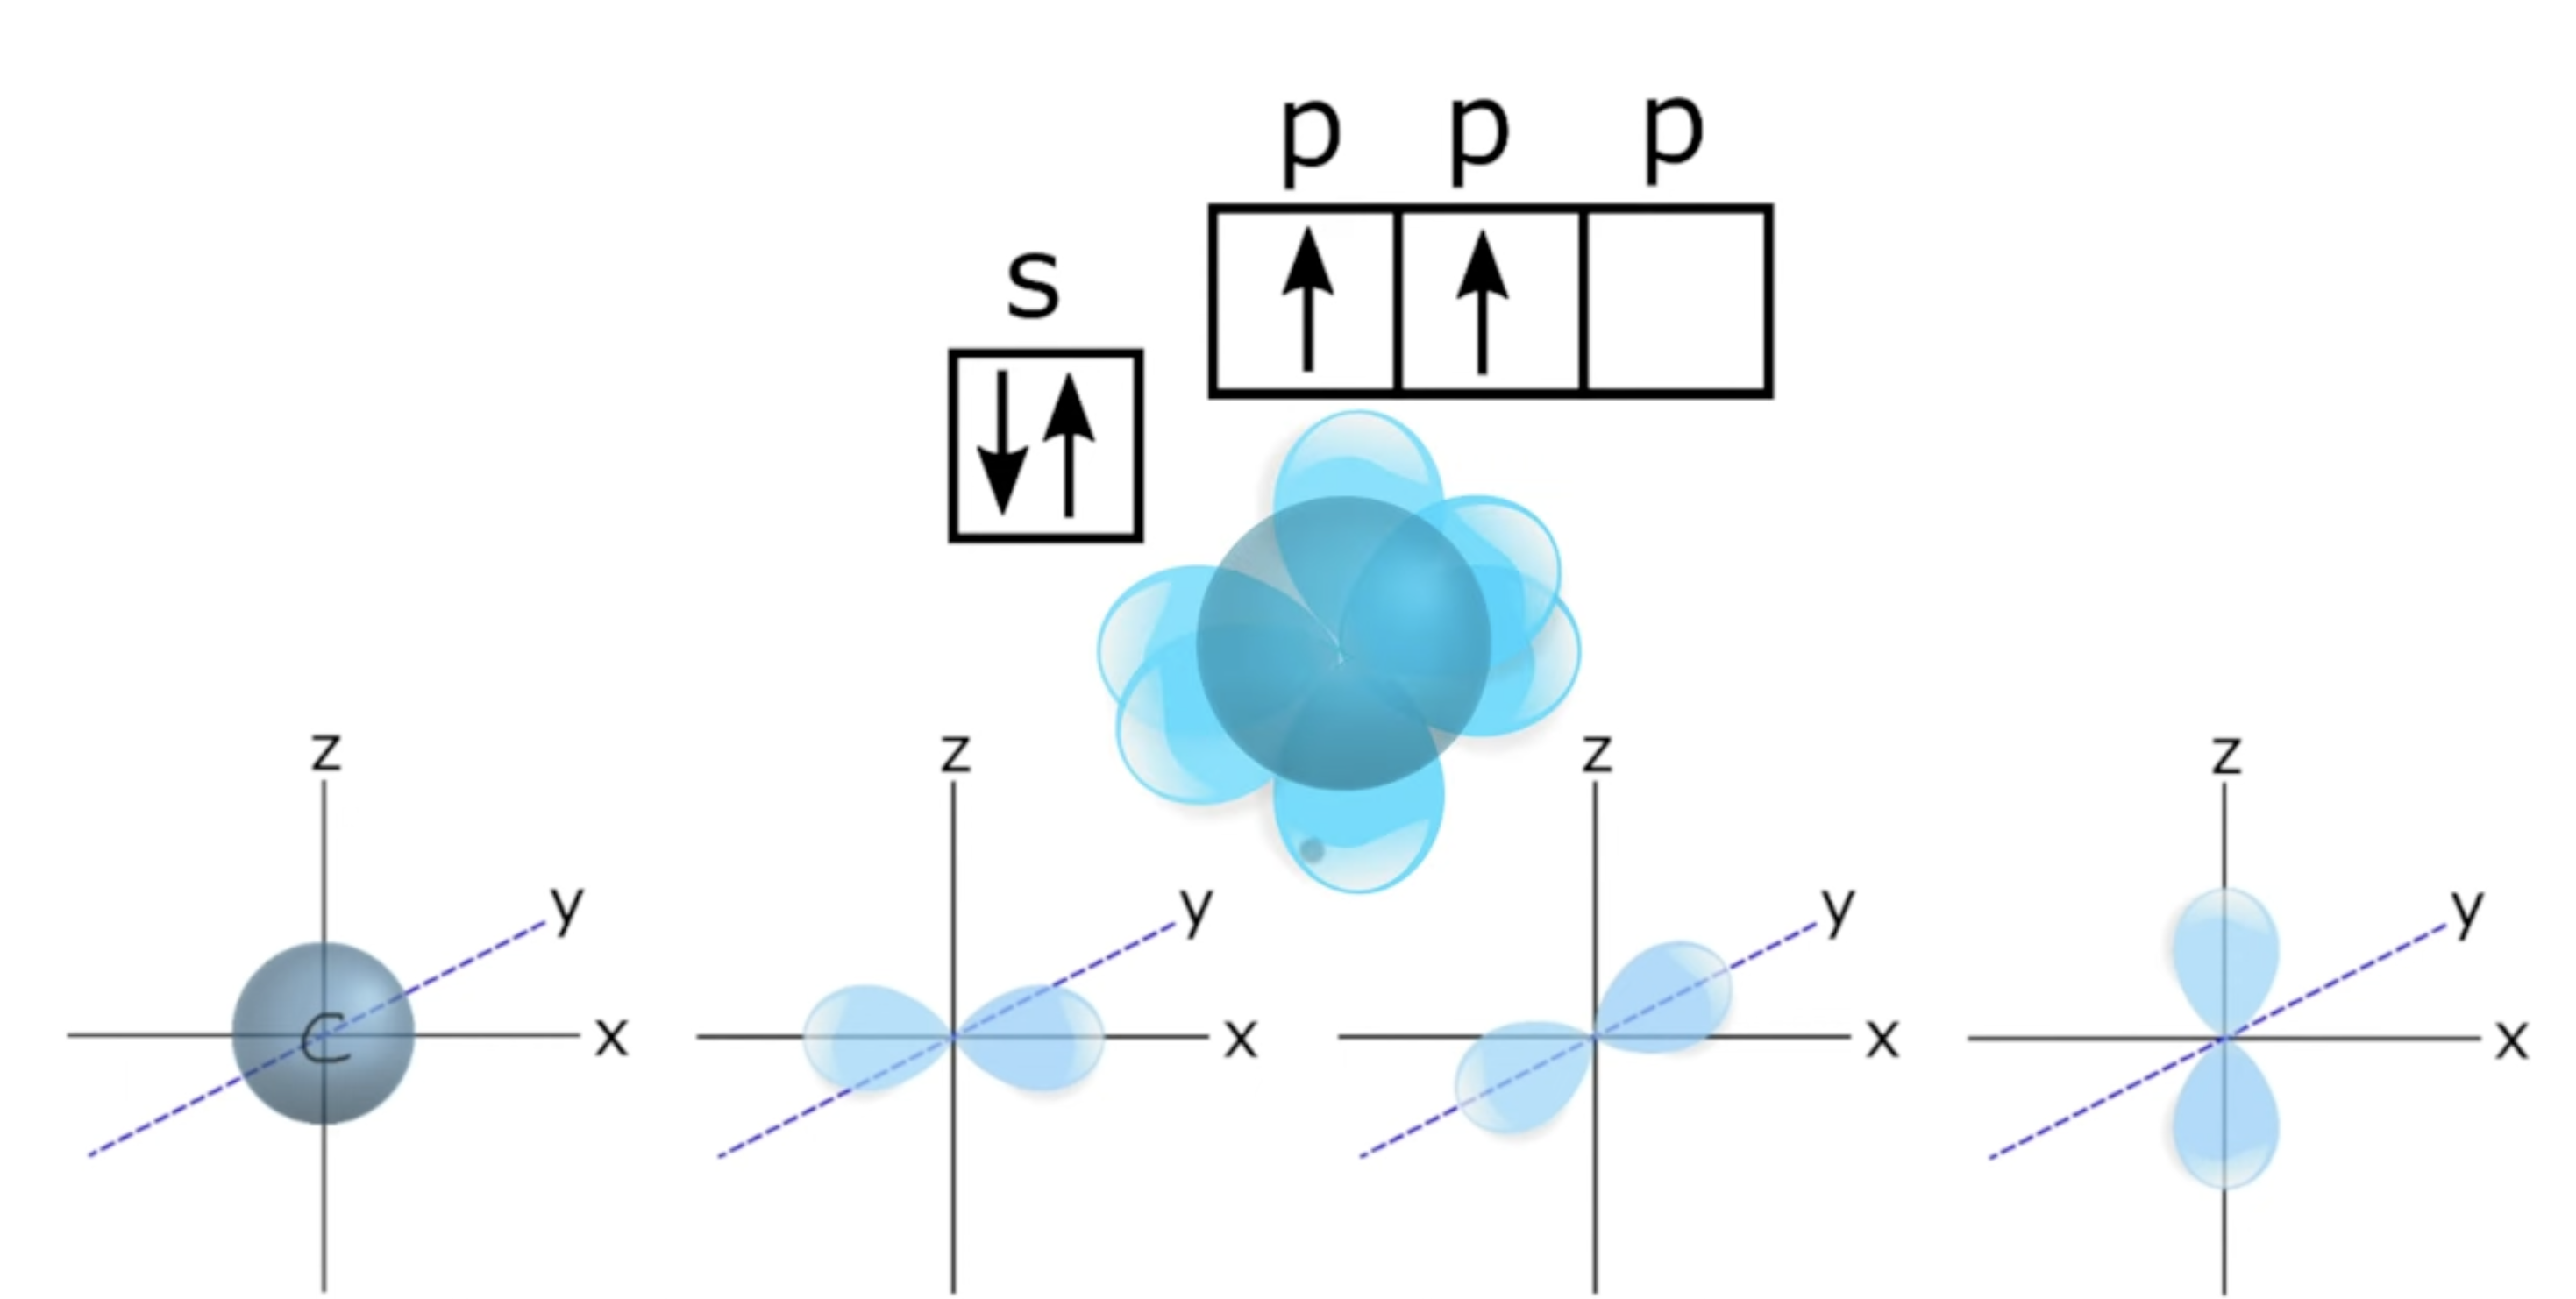
\includegraphics[width=0.65\textwidth]{ibridazione_carbonio.png}
  \caption{$sp^3$ hybridisation of carbon: the four equivalent hybrid orbitals orient tetrahedrally.}
\end{figure}

\begin{esempio}
\textbf{CH$_4$}: tetrahedral, $109{,}5°$.\quad \textbf{NH$_3$}: pyramidal, $107{,}3°$.\quad \textbf{H$_2$O}: bent, $105°$.
\end{esempio}

\subsection{$sp^2$ Hybridisation}

$1\,s + 2\,p \;\Rightarrow\; 3$ in-plane $sp^2$ orbitals ($120°$) + 1 perpendicular $p$ orbital $\Rightarrow$ 1 $\pi$ bond possible.

\begin{esempio}
\textbf{H$_2$C$=$CH$_2$}: planar, $120°$.
\end{esempio}

\subsection{$sp$ Hybridisation}

$1\,s + 1\,p \;\Rightarrow\; 2$ linear $sp$ orbitals ($180°$) + 2 pure $p$ orbitals $\Rightarrow$ up to 2 $\pi$ bonds.

\begin{esempio}
\textbf{HC$\equiv$CH}: linear, $180°$.
\end{esempio}

\subsection{Practical Rule: How to Determine Hybridisation}

\altrow
\begin{center}
\begin{tabular}{cclll}
\toprule
\rowcolor{epflred!85}
\textcolor{white}{\textbf{El.\ groups}} & \textcolor{white}{\textbf{Hybridisation}} & \textcolor{white}{\textbf{Electronic geometry}} & \textcolor{white}{\textbf{Free $p$ orb.}} & \textcolor{white}{\textbf{$\pi$ bonds}} \\
\midrule
2 & $sp$      & Linear              & 2 & up to 2 \\
3 & $sp^2$    & Trigonal planar     & 1 & 1 \\
4 & $sp^3$    & Tetrahedral         & 0 & 0 \\
5 & $sp^3d$   & Trigonal bipyramid. & -- & -- \\
6 & $sp^3d^2$ & Octahedral          & -- & -- \\
\bottomrule
\end{tabular}
\end{center}
\resetrow

\begin{attenzione}
\textbf{Multiple bond $\Rightarrow$ reduced hybridisation.} Double bond $\Rightarrow$ $sp^2$; triple bond $\Rightarrow$ $sp$.
\end{attenzione}

\vspace{4pt}
\altrow
\begin{center}
\begin{tabular}{lllll}
\toprule
\rowcolor{epflred!85}
\textcolor{white}{\textbf{Molecule}} & \textcolor{white}{\textbf{Hybrid.}} & \textcolor{white}{\textbf{Geometry}} & \textcolor{white}{\textbf{Angle}} & \textcolor{white}{\textbf{$\sigma$\,/\,$\pi$}} \\
\midrule
CH$_4$              & $sp^3$ & Tetrahedral      & $109{,}5°$ & 4$\sigma$, 0$\pi$ \\
NH$_3$              & $sp^3$ & Pyramidal        & $107{,}3°$ & 3$\sigma$, 0$\pi$ \\
H$_2$O              & $sp^3$ & Bent             & $105°$     & 2$\sigma$, 0$\pi$ \\
H$_2$C$=$CH$_2$     & $sp^2$ & Planar           & $120°$     & 5$\sigma$, 1$\pi$ \\
HC$\equiv$CH        & $sp$   & Linear           & $180°$     & 3$\sigma$, 2$\pi$ \\
CO$_2$              & $sp$   & Linear           & $180°$     & 2$\sigma$, 2$\pi$ \\
BF$_3$              & $sp^2$ & Trigonal planar  & $120°$     & 3$\sigma$, 0$\pi$ \\
\bottomrule
\end{tabular}
\end{center}
\resetrow

\end{document}
